\section{Exceptional Control Flow}

\begin{concept}{Exception Types}\\
Two main categories of exceptions:

\textbf{Interrupt Sources:}
\begin{itemize}
  \item Peripherals requesting immediate CPU attention
  \item Software-generated interrupts
  \item Asynchronous to instruction execution
\end{itemize}

\textbf{System Exceptions:}
\begin{itemize}
  \item \textbf{Reset}: Processor restart
  \item \textbf{NMI}: Non-maskable Interrupt (cannot be ignored)
  \item \textbf{Faults}: Undefined instructions, errors
  \item \textbf{System Calls}: OS services (SVC and PendSV)
\end{itemize}
\end{concept}

\begin{definition}{Interrupt Control}\\
PRIMASK register controls interrupt handling:
\begin{itemize}
  \item Single bit controls all maskable interrupts
  \item Reset state: PRIMASK = 0 (interrupts enabled)
  \item Control methods:
    \begin{itemize}
      \item Assembly: \texttt{CPSID i} (disable), \texttt{CPSIE i} (enable)
      \item C: \texttt{\_\_disable\_irq()}, \texttt{\_\_enable\_irq()}
    \end{itemize}
\end{itemize}

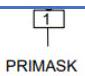
\includegraphics[width=\linewidth]{images/2024_12_29_79e6b22f503fb7b4f718g-11}
\end{definition}

\begin{definition}{Context Storage}\\
Interrupt handling requires automatic context saving:

\textbf{ISR Entry:}
\begin{itemize}
  \item Stores on stack:
    \begin{itemize}
      \item xPSR, PC, LR, R12
      \item R0-R3 (caller-saved registers)
    \end{itemize}
  \item Stores EXC\_RETURN in LR
\end{itemize}

\textbf{ISR Exit:}
\begin{itemize}
  \item Via BX LR or POP {..., PC}
  \item Restores from stack:
    \begin{itemize}
      \item R0-R3, R12, LR, PC
      \item xPSR
    \end{itemize}
\end{itemize}
\end{definition}

\begin{concept}{Polling vs Interrupts}\\
\textbf{Polling Approach:}
\begin{itemize}
  \item Periodic status register checks
  \item Synchronous with main program
  \item \textbf{Advantages:}
    \begin{itemize}
      \item Simple implementation
      \item Predictable timing
      \item No extra hardware needed
    \end{itemize}
  \item \textbf{Disadvantages:}
    \begin{itemize}
      \item CPU wastes time waiting
      \item Reduced system throughput
      \item Longer response times
    \end{itemize}
\end{itemize}

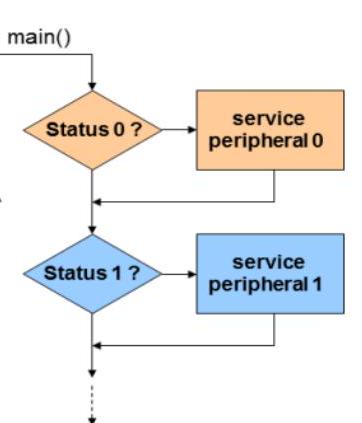
\includegraphics[width=\linewidth]{images/2024_12_29_79e6b22f503fb7b4f718g-11(1)}

\textbf{Interrupt Approach:}
\begin{itemize}
  \item Hardware-triggered event handling
  \item Asynchronous to main program
  \item \textbf{Advantages:}
    \begin{itemize}
      \item Efficient CPU usage
      \item Quick response times
      \item Better system throughput
    \end{itemize}
  \item \textbf{Disadvantages:}
    \begin{itemize}
      \item More complex implementation
      \item Harder to debug
      \item Timing less predictable
    \end{itemize}
\end{itemize}

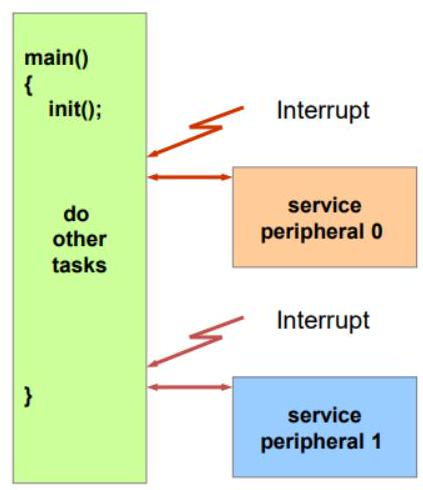
\includegraphics[width=\linewidth]{images/2024_12_29_79e6b22f503fb7b4f718g-11(2)}
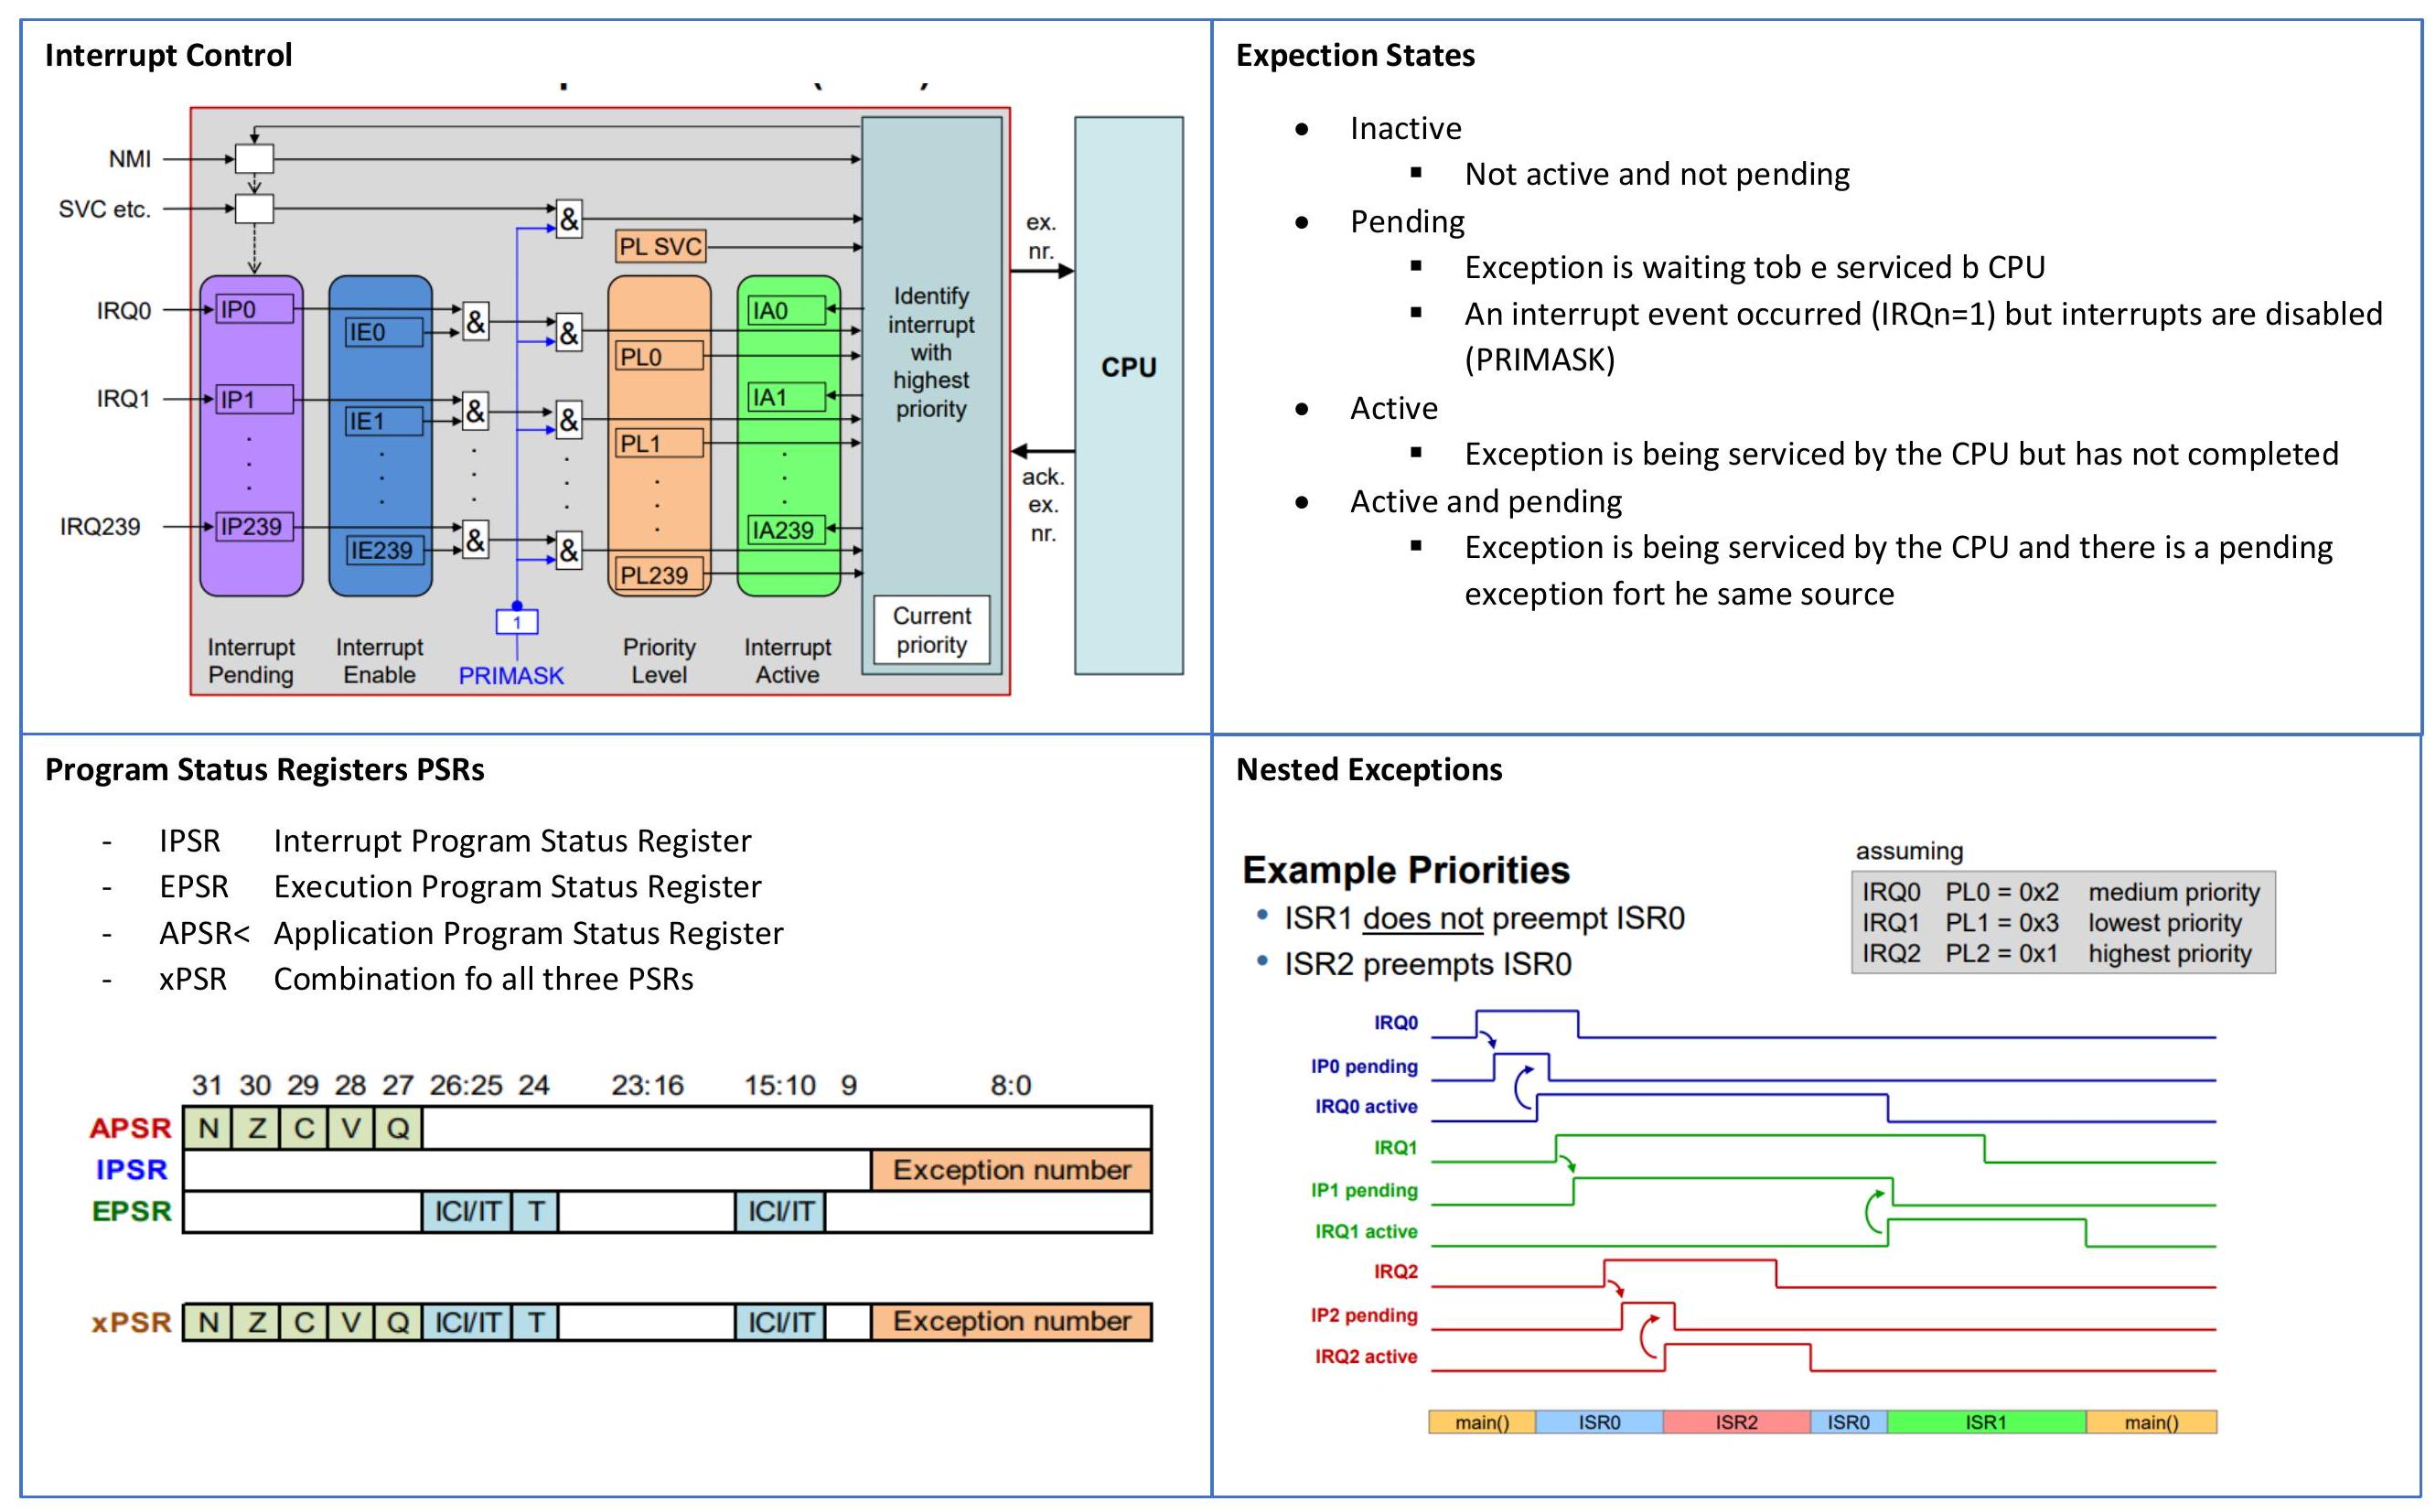
\includegraphics[width=\linewidth]{images/2024_12_29_79e6b22f503fb7b4f718g-12}
\end{concept}

\begin{example2}{Basic ISR Implementation}
\begin{lstlisting}[language=armasm, style=basesmol]
    ; Interrupt Service Routine
    EXPORT MyISR
MyISR
    PUSH    {R4-R7, LR}    ; Save registers
    
    ; Handle interrupt here
    ; R0-R3 already saved automatically
    
    POP     {R4-R7, PC}    ; Restore and return
\end{lstlisting}
\end{example2}

\begin{KR}{Implementing Interrupt Handlers}\\
Steps for implementing interrupt handlers:
\begin{enumerate}
  \item Define interrupt vector
  \item Save necessary context
  \item Handle the interrupt
  \item Clear interrupt flag
  \item Restore context
  \item Return from interrupt
\end{enumerate}

Important considerations:
\begin{itemize}
  \item Keep ISRs short
  \item Handle critical tasks only
  \item Be aware of nested interrupts
  \item Protect shared resources
\end{itemize}
\end{KR}

\begin{concept}{NVIC (Nested Vectored Interrupt Controller)}\\
Key components and functionality:
\begin{itemize}
  \item \textbf{Interrupt States}:
    \begin{itemize}
      \item \textbf{Inactive}: Not active and not pending
      \item \textbf{Pending}: Waiting to be serviced
      \item \textbf{Active}: Currently being serviced
      \item \textbf{Active and Pending}: Being serviced with new request
    \end{itemize}
  \item \textbf{Control Registers}:
    \begin{itemize}
      \item Interrupt Enable (IE)
      \item Interrupt Pending (IP)
      \item Interrupt Active (IA)
      \item Priority Level (PL)
    \end{itemize}
\end{itemize}

%\includegraphics[width=\linewidth]{images/2024_12_29_79e6b22f503fb7b4f718g-11(3)}
\end{concept}

\begin{formula}{Interrupt Control Registers}\\
Important NVIC registers:

1. Enable/Disable Registers:
\begin{lstlisting}[language=armasm, style=base]
SETENA0 EQU 0xE000E100    ; Enable interrupts
CLRENA0 EQU 0xE000E180    ; Disable interrupts

; Enable IRQ3
LDR     R0, =SETENA0
MOVS    R1, #(1<<3)
STR     R1, [R0]

; Disable IRQ3
LDR     R0, =CLRENA0
MOVS    R1, #(1<<3)
STR     R1, [R0]
\end{lstlisting}

2. Pending Registers:
\begin{lstlisting}[language=armasm, style=base]
SETPEND0 EQU 0xE000E200   ; Set pending
CLRPEND0 EQU 0xE000E280   ; Clear pending

; Set IRQ3 pending
LDR     R0, =SETPEND0
MOVS    R1, #(1<<3)
STR     R1, [R0]

; Clear IRQ3 pending
LDR     R0, =CLRPEND0
MOVS    R1, #(1<<3)
STR     R1, [R0]
\end{lstlisting}
\end{formula}

\begin{concept}{Priority System}\\
Interrupt priority handling:
\begin{itemize}
  \item \textbf{Priority Levels}:
    \begin{itemize}
      \item 0-255 (lower number = higher priority)
      \item Fixed priorities for system exceptions
      \item Programmable priorities for IRQs
    \end{itemize}
  \item \textbf{Preemption}:
    \begin{itemize}
      \item Higher priority interrupts can preempt lower
      \item Same priority follows FIFO
    \end{itemize}
\end{itemize}

Example priority setting:
\begin{lstlisting}[language=C, style=base]
// Set priority for IRQ3
NVIC_SetPriority(IRQ3_IRQn, 2);

// Get priority
uint32_t prio = NVIC_GetPriority(IRQ3_IRQn);
\end{lstlisting}
\end{concept}

\begin{KR}{Exception Vector Table}\\
Setup and usage:

1. Vector table structure:
\begin{lstlisting}[language=armasm, style=base]
    AREA RESET, DATA, READONLY
__Vectors
    DCD     __initial_sp        ; Top of Stack
    DCD     Reset_Handler       ; Reset
    DCD     NMI_Handler        ; NMI
    DCD     HardFault_Handler  ; Hard Fault
    DCD     0                  ; Reserved
    DCD     0                  ; Reserved
    DCD     0                  ; Reserved
    ; ... more vectors
    DCD     IRQ0_Handler       ; IRQ0
    DCD     IRQ1_Handler       ; IRQ1
\end{lstlisting}

2. Handler implementation:
\begin{lstlisting}[language=armasm, style=base]
    AREA |.text|, CODE, READONLY
    
IRQ0_Handler PROC
    EXPORT IRQ0_Handler
    PUSH    {R4-R7,LR}
    ; Handle interrupt
    POP     {R4-R7,PC}
    ENDP
\end{lstlisting}
\end{KR}

\begin{example2}{Nested Interrupts Example}
Implementation with different priorities:
\begin{lstlisting}[language=C, style=base]
// Initialize interrupts
void init_interrupts(void) {
    // Enable interrupts
    NVIC_EnableIRQ(IRQ0_IRQn);
    NVIC_EnableIRQ(IRQ1_IRQn);
    
    // Set priorities
    NVIC_SetPriority(IRQ0_IRQn, 1); // Higher
    NVIC_SetPriority(IRQ1_IRQn, 2); // Lower
    
    // Enable global interrupts
    __enable_irq();
}

// Higher priority ISR
void IRQ0_Handler(void) {
    // Handle high priority interrupt
    // Can't be interrupted by IRQ1
}

// Lower priority ISR
void IRQ1_Handler(void) {
    // Handle low priority interrupt
    // Can be interrupted by IRQ0
}
\end{lstlisting}
\end{example2}

\begin{concept}{Data Consistency}\\
Handling shared data access:
\begin{itemize}
  \item \textbf{Race Conditions}:
    \begin{itemize}
      \item Main program and ISR accessing same data
      \item Interrupts during multi-step operations
    \end{itemize}
  \item \textbf{Solutions}:
    \begin{itemize}
      \item Disable interrupts during critical sections
      \item Use atomic operations
      \item Implement proper synchronization
    \end{itemize}
\end{itemize}

Example protection:
\begin{lstlisting}[language=C, style=base]
void update_shared_data(void) {
    __disable_irq();         // Critical section start
    shared_var++;           // Update shared data
    __enable_irq();         // Critical section end
}
\end{lstlisting}
\end{concept}

\begin{KR}{CMSIS Functions for Interrupt Control}\\
Standard CMSIS functions for interrupt handling:
\begin{itemize}
  \item \texttt{NVIC\_EnableIRQ(IRQn)}: Enable specific interrupt
  \item \texttt{NVIC\_DisableIRQ(IRQn)}: Disable specific interrupt
  \item \texttt{NVIC\_SetPendingIRQ(IRQn)}: Set interrupt pending
  \item \texttt{NVIC\_ClearPendingIRQ(IRQn)}: Clear pending status
  \item \texttt{NVIC\_SetPriority(IRQn, priority)}: Set priority
  \item \texttt{NVIC\_GetPriority(IRQn)}: Read priority
\end{itemize}

Example usage:
\begin{lstlisting}[language=C, style=base]
void init_timer_interrupt(void) {
    // Enable timer interrupt
    NVIC_EnableIRQ(TIM2_IRQn);
    
    // Set priority
    NVIC_SetPriority(TIM2_IRQn, 2);
    
    // Configure timer
    // ...
    
    // Enable global interrupts
    __enable_irq();
}
\end{lstlisting}
\end{KR}